% this file is called up by thesis.tex
% content in this file will be fed into the main document

%: ----------------------- name of chapter  -------------------------
\chapter{Moduli varieties and their tangent spaces}\label{chap:moduli}


%: ----------------------- paths to graphics ------------------------

% change according to folder and file names
\ifpdf
    \graphicspath{{figures/PNG/}{figures/}{figures/}}
\else
    \graphicspath{{figures/EPS/}{figures/}}
\fi

%: ----------------------- contents from here ------------------------


In this Chapter we give a scheme-theoretic definition of the moduli varieties $\Xdr$ parametrizing effective divisors and $\Wdr$ parametrizing linear series. The idea is to start from the two free presentations \eqref{eq:univ_div_seq} and \eqref{eq:univ_lb_seq} of the sheaves $R^1 \pi_* \calO_Z(\Delta)$ and $R^1 \nu_{*} \scL$ arising from some specific cohomology sequences related to the universal divior $\Delta$ and the universal line bundle $\scL$.\\
Then we introduce the concept of Fitting ideals, which is at the heart of this technical -- but extremely useful -- approach. Fitting ideals enjoy nice scheme-theoretical properties and, consequently, the scheme structure that we get on the moduli varieties turns out to be satisfactory for different reasons. For instance, Proposition \ref{prop:scheme_theo_inv_img} shows that the obvious set-theoretic identity $\Xdr = u^{-1}(\Wdr)$ holds in the category of schemes.\\
As a consequence of our definitions, it will be possible to exploit a Theorem on the height of Fitting ideals, proved by Eagon and Northcott, to give a lower bound to the dimension of the moduli varieties \moduu in terms of the \BN number $\rho$. \\
Next we will introduce the variety $G_d^r$ parametrizing (not necessarily complete) linear series which, in the following Section, will permit to achieve a completely cohomological description of the tangent spaces of \modu, in which the Petri's map 
$$ \mu_0: H^0(D)\otimes H^0(K-D) \tolong H^0(K) $$ 
will turn out to play a crucial role. Relying on this description we will be able to characterize the smoothness of the moduli varieties.


\section{Fitting ideals and degeneracy loci}\label{sec:fitt_deg}
	
	Given a linear map $\ph:V\to W$ between finite dimensional vector spaces, one can look at its rank to get information about the \emph{amount of degeneracy} involved in the mapping. 
	More precisely, the lower the rank of $\ph$ is, the bigger the dimension of its fibres will be or, in other words, more \emph{directions} in $V$ will be collapsed. 
	Moreover, if the map and the vector spaces depend on some parameters $x = x_1,\dots, x_n$, one can define the locus where the rank of $\ph(x)$ is at most $t$, what is usually referred to as the $t$-\textbf{degeneracy locus} of $\ph$.\\
	%
	\begin{comment}
		For instance, let $f$ be a morphism $M\to N$ of two varieties and think of the parameters as local coordinates on $M$. Then the tangent map of $f$ can be thought, locally, as a bunch of linear maps $df_x:T_x M \to T_{f(x)} N$ and, if the rank of $df_x$ is not maximal at a point $P=P(x)$, this means $f$ is constant in one or more directions around $P$ or, in other words, the morphism is collapsing part of $M$ to a variety of lower dimension.
		\begin{figure}[ht]
			\centering
			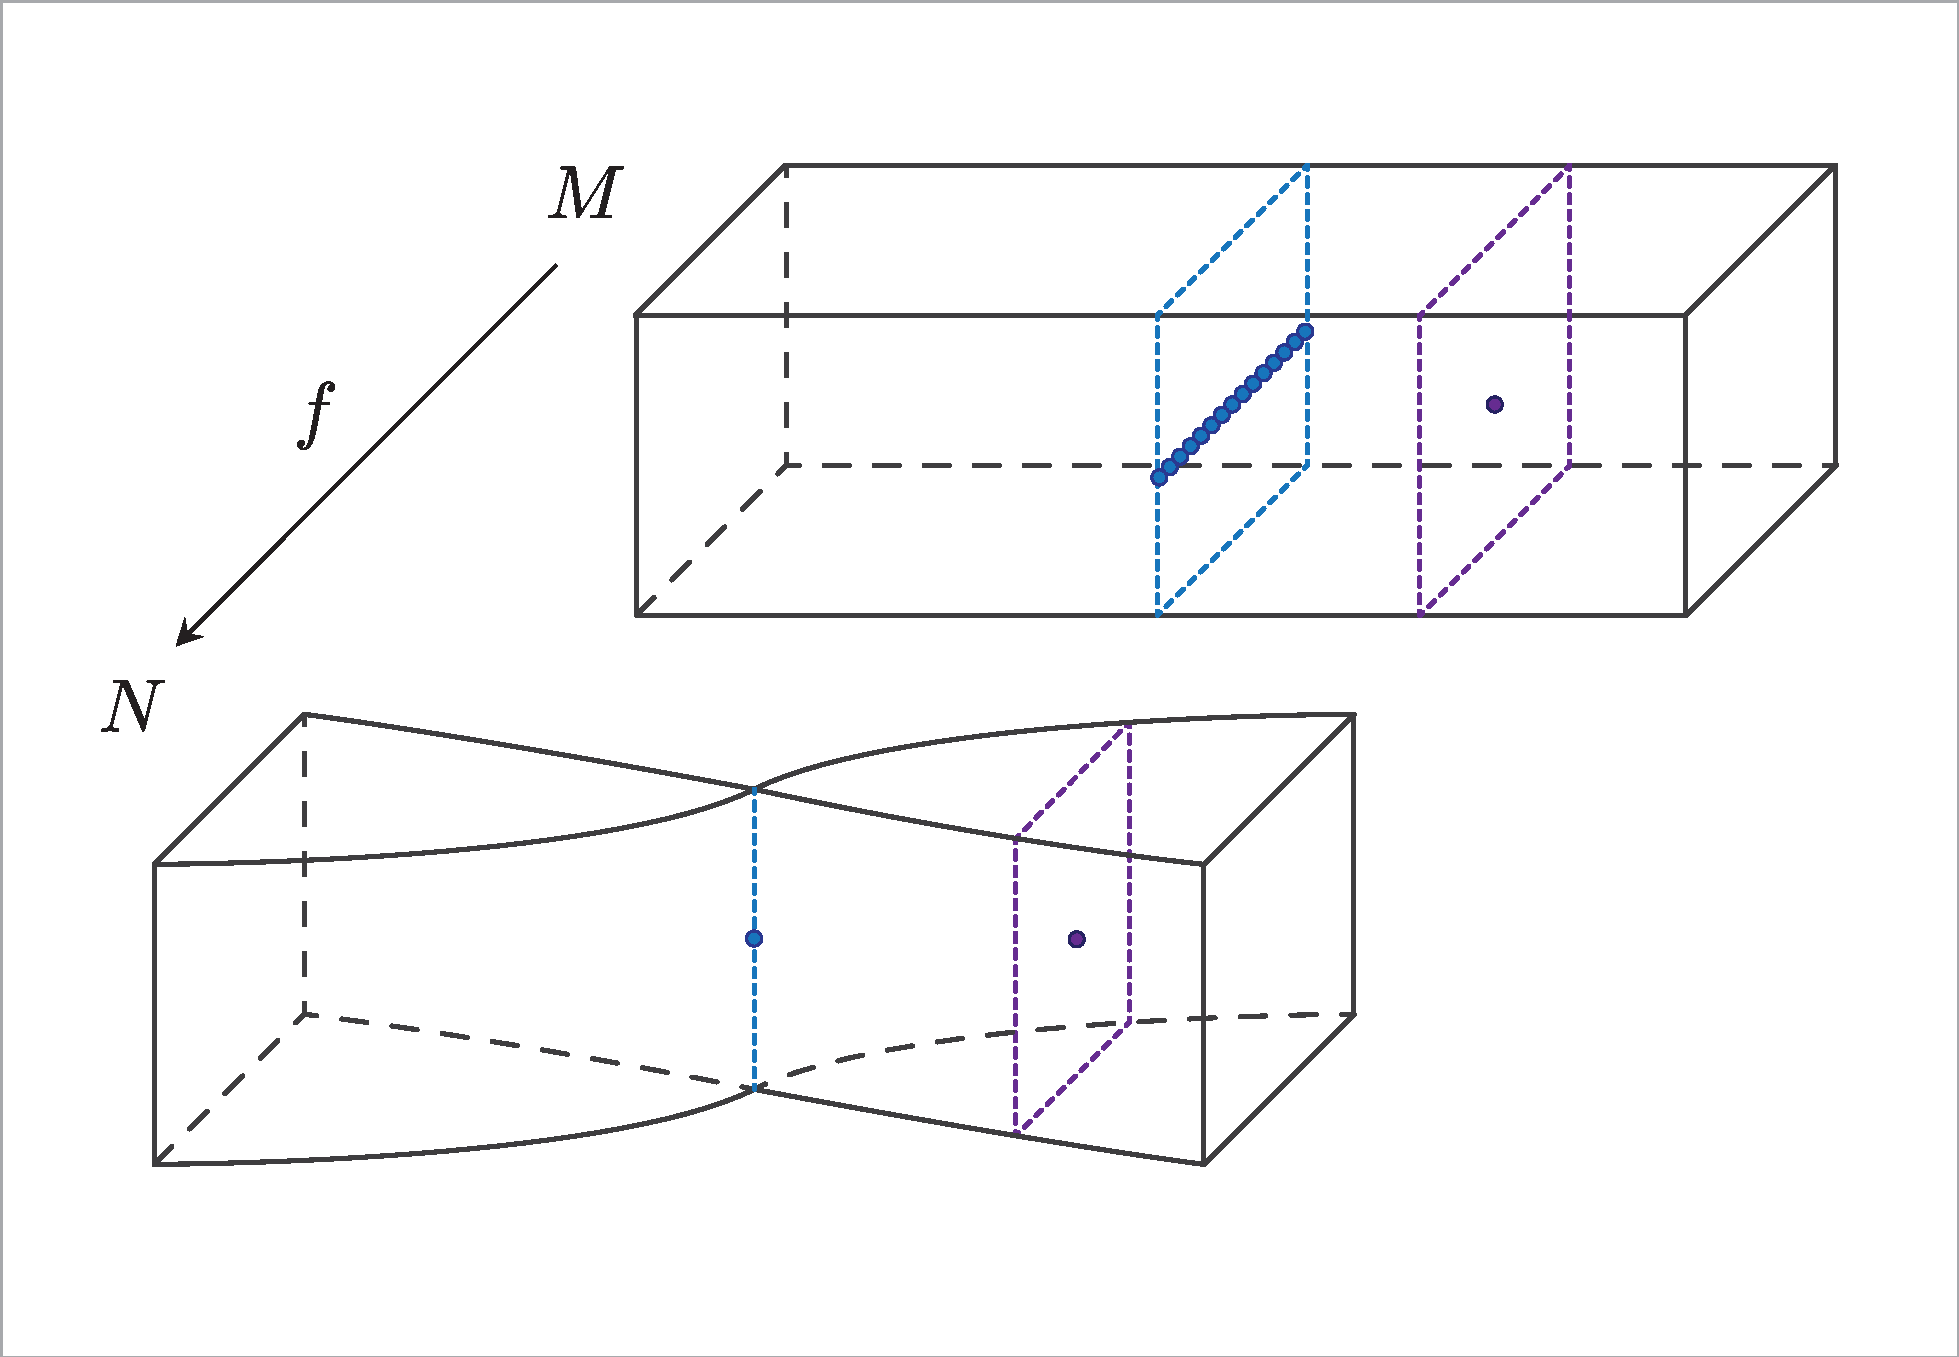
\includegraphics[width=0.85\textwidth]{Degeneracy2.pdf}
			\caption{An example of degeneration of a morphism between varieties }
		\end{figure}
	\end{comment}
	In our case we work in a more general setting: we consider a morphism between two locally free sheaves of finite type, but the underlying intuition is similar.\\

	Let $\ph:E\to F$ be a morphism of locally free sheaves of finite ranks $e$ and $f$ over a Noetherian scheme $Y$ and $n \leq \min(e,f)$. We are interested in studying the $(n-1)$-\textbf{degeneracy locus} of $\ph$, which is defined as
	$$ D_{n-1} (\ph) = \set{ y\in Y \mid \rank_y(\ph) < n }. $$
	Since we want to work with degeneracy loci, it is useful to define the ideal $I_n(\ph)$, generated by all of the $n\times n$ minors of $\ph$. This can be done in a coordinate-free way through the formalism of exterior algebra:
	\begin{defi}
	Let $\ph:E\to F$ be a map of free modules over a ring $R$. We define the ideal $I_n(\ph) \subset R$ to be the image of the canonical map induced by $\ph$ 
	$$ \wedge^n E \otimes\wedge^n F^*\to R. $$
	\end{defi}
	\begin{rema}
		The canonical map involved in the definition of $I_n(\ph)$ is obtained in the following way: first, by the universal property of exterior algebra, given $\nobreak{\ph:E\to F}$ we have a unique map
		$$ \wedge^n\ph : \wedge^n E \to \wedge^n F $$
		and we can thus define the above canonical map as
		$$ \wedge^n E \otimes\wedge^n F^*\to R, \qquad a\otimes b \mapsto b(\wedge^n\ph(a)) $$
	\end{rema}

	Next we introduce the concept of the $n$-th Fitting ideal associated to to a finitely presented module. This is a powerful algebraic invariant, which will serve us to define the moduli varieties \moduu parametrising effective divisors and linear series.

	\begin{defi}
		Let $G$ be a finitely presented module over a ring $R$ and consider a free presentation 
		$$ E \overset{\ph}\to F \to G \to 0 $$ of $G$ such that $F$ is a finitely generated $R$-module of rank $f$. For every integer
		$t \in \N$ we define the $t$-th \textbf{Fitting ideal} of $G$ to be 
		$$ \Fitt_t(G) := I_{f-t}(\ph). $$
	\end{defi}

	\begin{rema}
	Fitting ideals are well-defined, since $\Fitt_t(G)$ does not depend on the chosen presentation. More precisely, if we have another presentation
			$$ E' \overset{\ph'}\to F' \to G \to 0 $$
			with $F'$ of rank $f'$ then $I_{f-t}(\ph) = I_{f'-t}(\ph') $, as it was proved by Hans Fitting in his paper \cite{FITT} of 1936.
	\end{rema}
	The above remark allow us to extend the definition to quasicoherent sheaves over a scheme.
	\begin{defi}
		Let ${G}$ be a locally-free coherent sheaf over a Noetherian scheme $Y$. We have local free presentations of ${G}$ over an open cover of $Y$ and, due to the above remark, the local $t$-th Fitting ideals fit together into a globally defined sheaf of ideals on $Y$, which we denote by $\Fitt_t({G}) \subset \calO_Y$.\\
		Since the ideal sheaf $\Fitt_t({G})$ is coherent by construction, it cuts out a closed subscheme of $Y$ which we denote by $ \FittS_t({G}) $, the $t$-\textbf{Fitting scheme} of ${G}$.
	\end{defi}
	Another useful property of Fitting ideals is their \textbf{invariance under base change}. More precisely, for every morphism of schemes $f:Y'\to Y$, the pullback of the Fitting ideal $f^*\Fitt_t({G})$ is generated as an $\calO_{Y'}$-module by the Fitting ideal of the pullback $\Fitt_t(f^*{G})$.\\
	
	Finally we define the locus of points $y$ where the fibers of $\ph_y$ have a certain dimension:
	\begin{defi}
		Let $m\in \N$ and $\ph:E\to F$ be a morphism of locally free sheaves over a Noetherian scheme $Y$. We define the set
		$$ \Fib_m (\ph) = \set{ y\in Y \mid \text{ fibers of } \ph_y \text{ have dimension } \geq m } $$
	\end{defi}
	Notice that, if $s\in \N$ and we have a free presentation of a coherent sheaf $G$
	$$ E\overset{\ph}\to F \to G\to 0 $$
	with $E$ of rank $e$ and $F$ of rank $f$, then it is a trivial consequence of the definitions that there is the following set-theoretic relationship among the objects we just defined:
	\begin{equation}\label{eq:degeneracy}
		\Supp\left[\,\FittS_{(s-1)}(G)\,\right] = D_{(f-s)}(\ph) = \Fib_{(e-f+s)}(\ph).
	\end{equation}
	

\section{Definition of \modu}\label{sec:defi_modu}
	%
	In order to define $\Xdr$ and $\Wdr$ -- the varieties parametrising linear series -- we will consider the free presentation appearing in Proposition \ref{prop:free_pres}, namely
	$$ 
	\pi_* \calO_{\Delta}(\Delta)\overset{\delta}\tolong R^1 \pi_* \calO \tolong R^1 \pi_* \calO(\Delta) \tolong 0 
	$$
	arising naturally from the universal divisor $\Delta$ and, further, the free presentation
	$$ 
	\nu_{*} \scL(\Gamma)\tolong \nu_{*} \scL(\Gamma) / \scL \tolong R^1 \nu_{*} \scL \tolong 0
	$$
	associated to the universal line bundle $\scL$.
	As we explained in Chapter \ref{chap:relative_Pic_and_Div}, the first of the above presentations -- which lives over $X\times \Dd$ -- is related to the tangent map of the Abel-Jacobi map $u$ and thus embeds information on its degeneracy loci. 
	Further, in Proposition \ref{prop:scheme_theo_inv_img} we will show that the second one -- which lives over $X\times \Pd$ -- encodes basically the same information \emph{modulo linear equivalence} and in fact pulls back to the first one, via $u$. 
	For these reasons we will use the schemes associated to some specific Fitting ideals of these presentations to define \modu.
	\begin{defi}
		We define
		$$ \Xdr := \FittS_{(g-d+r-1)}(R^1\pi_* \calO(\Delta)) \AND  \Wdr := \FittS_{(g-d+r-1)}(R^1\nu_{*} \scL) $$
	\end{defi}
	As a preparation for the next Proposition we need the following Lemma, which illustrates in what precise sense the sequence \eqref{eq:univ_lb_direct_image} associated to the universal divisor is functorial.
	\begin{lemm}\label{lemm:functoriality}
		Let $L$ be a line bundle of degree $d$ on $X\times T$ and let $f:T\to \Pd$ the unique map for which
		$$ f^*\scL \cong L \otimes \phi^* F $$
		where $F$ is a line bundle over $T$ and $\phi: X\times T \to T$ is the natural projection. Further, let $\Gamma':= \phi^* M$ where $M$ is a divisor of high degree $m$ as defined in \ref{def:Gamma}.
		Then the sequence \eqref{eq:univ_lb_direct_image} pulls back via $f$ to the exact sequence
		$$ 0 \to \phi_*L\otimes F  \to \phi_* L(\Gamma')\otimes F \to \phi_* (L(\Gamma') / L)\otimes F  \to R^1 \phi_* L\otimes F  \to 0 $$ 
	\end{lemm}
	\begin{rema}
		Before starting with the proof let us remark that, given a family of line bundles $L$ as in the above statement, we have an exact sequence which is very similar to \eqref{eq:univ_lb_direct_image}. Indeed, since $\Gamma'$ is the pullback of a divisor of high degree on $X$, Lemma \ref{lemm:trivial_R1} implies $R^1\phi_* L(\Gamma') = 0$. Therefore, considering the natural \ses 
		$$ \SES{L}{L(\Gamma')}{L(\Gamma')/L} $$
		and taking the direct image through $\phi$ we obtain the exact sequence
		$$ 0 \to \phi_*L  \to \phi_* L(\Gamma') \to \phi_* (L(\Gamma') / L)  \to R^1 \phi_* L  \to 0\;. $$
	\end{rema}
	\begin{proof}
		First of all we notice that the locally free sheaf $\scL(\Gamma)$ enjoys the following properties 
		\begin{itemize}
			\item $\nu_{*} \scL(\Gamma)$ is locally free, as showed in Proposition \ref{prop:free_pres}
			\item $R^i \nu_{*} \scL(\Gamma) = 0$ for every $i\geq 1$, as proven in Lemma \ref{lemm:trivial_R1}
		\end{itemize}
		Hence we can apply Proposition \ref{prop:R1_trick} to the base change diagram
		$$
		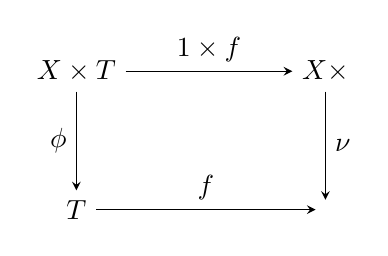
\begin{tikzpicture}[node distance=5em, auto]
			\node (A) 															{$X\times T$};
			\node (B) 	[right of=A, xshift=4em]		{$X\times \Pd$};
		  \node (C) 	[below of=A]	 							{$T$};
		  \node (D) 	[below of=B] 								{$\Pd$};
		  \draw[-stealth] 				(A)		to node {$1\times f$} (B);
		  \draw[-stealth]					(C)		to node {$f$} 				(D);
		  \draw[-stealth][swap]		(A)		to node {$\phi$} 			(C);
		  \draw[-stealth]					(B)		to node {$\nu$} 			(D);
		\end{tikzpicture}
		$$
		and, using the Projection Formula \eqref{eq:proj_formula}, we deduce that there is a natural isomorphism
		\begin{equation}
			f^* R^1 \nu_{*} \scL(\Gamma) \cong  R^1 \pi_* f^* \scL(\Gamma) \cong R^1 \pi_* (L(\Gamma')\otimes \phi^*F ) \cong R^1 \pi_* L(\Gamma') \otimes F \,.
		\end{equation}
		Moreover, during the proof of Proposition \ref{prop:free_pres} we showed that $\nu_{*} \scL(\Gamma)/\scL $ is also locally free and, further, from the exactness of the direct image sequence
		$$ 
			\dots \to R^1 \nu_{*} \scL \to 0 \to R^1 \nu_{*} \scL(\Gamma)/\scL \to 0 \to \dots
		$$
		we see that $R^i \nu_{*} \scL(\Gamma)/\scL = 0$ for every $i\geq 1$ and, therefore, another application of Proposition \ref{prop:R1_trick} together with the projection formula gives us the natural isomorphism
		$$
			f^* R^1 \nu_{*} \scL(\Gamma)/\scL \; \cong \;  R^1 \pi_* L(\Gamma')/L \otimes F \,.
		$$
		As a result, recalling that \emph{tensoring with a line bundle} is an exact functor, we get the commutative diagram
		$$
		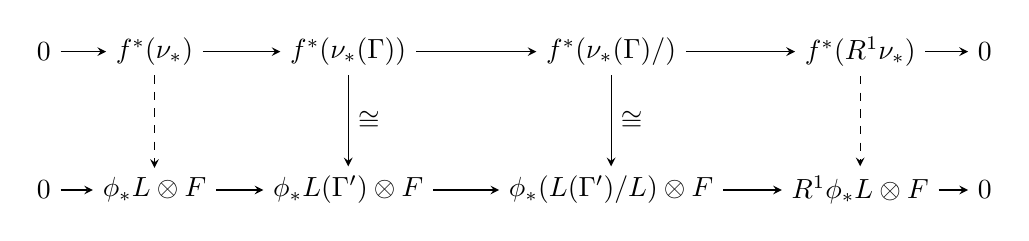
\begin{tikzpicture}[node distance=8em, auto]
			\node (O) 																{$0$};
			\node (A) 	[right of=O, xshift=-4em]			{$f^* (\nu_{*}\scL)$};
			%node (A2) 	[right of=A]									{$\;$};
			\node (B) 	[right of=A, xshift=-1em]			{$f^* (\nu_{*} \scL(\Gamma))$};
			%node (B2) 	[right of=B]									{$\;$};
		  \node (C) 	[right of=B, xshift=1.5em] 		{$f^* (\nu_{*} \scL(\Gamma)/\scL)$};
			%\node (C2) 	[right of=C]						 		{$\;$};
		  \node (D) 	[right of=C, xshift=1em] 			{$f^* (R^1 \nu_{*} \scL)$};
			\node (OO) 	[right of=D, xshift=-3.5em] 	{$0$};
		  \node (O') 	[below of=O,  yshift=3em] 		{$0$};
		  \node (A') 	[below of=A,  yshift=3em] 		{$\phi_*L\otimes F$};
		  \node (B') 	[below of=B,  yshift=3em] 		{$\phi_* L(\Gamma')\otimes F$};
		  \node (C') 	[below of=C,  yshift=3em] 		{$\phi_* (L(\Gamma') / L)\otimes F$};
		  \node (D') 	[below of=D,  yshift=3em] 		{$R^1 \phi_* L\otimes F$};
			\node (OO') [below of=OO, yshift=3em] 		{$0$};
			%
			\draw[-stealth] 					(O)		to node {} 				(A);
		  \draw[-stealth]						(A)		to node {} 				(B);
		  \draw[-stealth]						(B)		to node {} 				(C);
		  \draw[-stealth]						(C)		to node {} 				(D);
			\draw[-stealth]						(D)		to node {} 				(OO);
			\draw[-stealth] 					(O')	to node {} 				(A');
		  \draw[-stealth]						(A')	to node {} 				(B');
		  \draw[-stealth]						(B')	to node {} 				(C');
		  \draw[-stealth]						(C')	to node {} 				(D');
			\draw[-stealth]						(D')	to node {} 				(OO');		  
		  \draw[-stealth][dashed]		(A)		to node {} 				(A');
			\draw[-stealth]						(B)		to node {$\cong$} (B');
		  \draw[-stealth]						(C)		to node {$\cong$} (C');
		  \draw[-stealth][dashed]		(D)		to node {} 				(D');
		\end{tikzpicture}
		\vspace{0em}
		$$
		where of course the dashed arrows are also isomorphisms.
	\end{proof}
	For future reference, we remark the following obvious consequence of the above Lemma.
	\begin{coro}\label{coro:functoriality}
		In the situation of the above Lemma, we have a natural isomorphism
		$$ f^* R^1 \nu_{*} \scL \;\cong\;  R^1 \phi_* L \otimes F $$
	\end{coro}
	The following proposition will clarify the relationship between $\Xdr$ and $\Wdr$, showing that $\Xdr$ is the scheme-theoretical inverse image of $\Wdr$. 
	\begin{prop}\label{prop:scheme_theo_inv_img}
		The scheme theoretic inverse image of the variety $\Wdr$ via the Abel-Jacobi map equals $\Xdr$. In symbols this amounts to
		$$ u^{-1}(\Wdr) = \Xdr. $$
	\end{prop}
	\begin{proof}
		We remarked already that Fitting ideals are stable under base change and this implies in particular that, for any sheaf $\scr{F}$, $u^*\Fitt(\scr{F})$ is generated as a module by $\Fitt(u^*\scr{F})$. Therefore the ideal sheaf of $u^{-1}(\Wdr)$ is generated by $\Fitt(u^* R^1\nu_{*}\scL)$ and thus it is enough to show that the latter is isomorphic to $\Fitt(R^1\pi_* \calO(\Delta))$. To begin, pick $D\in \Dd$ and notice that the canonical maps
		$$ f: D \into \Dd \AND g: \calO(D)\into \Pd $$
		satisfy the relation $g = u\circ f$. So fiberwise we have the identities
		$$ (u^* \scL)_{\mid D} = f^* u^* \scL = (u\circ f)^* \scL = g^* \scL = \calO(D) = \calO(f^* \Delta) = f^*\calO(\Delta) = \calO(\Delta)_{\mid D} $$
		and we can therefore apply Lemma \ref{lemm:square} to get a line bundle $F$ over $\Dd$ such that
		$$ u^* \scL \;\cong\; \calO(\Delta) \otimes \pi^* F \,, $$
		where $\pi: X\times \Dd \to \Dd$ is the natural projection map. Finally, from Corollary \ref{coro:functoriality} we get a natural isomorphism
		$$ u^*  R^1\nu_{*}\scL \;\cong\; R^1\pi_*\calO(\Delta)\otimes F $$
		and, since $\square\otimes F$ is a right-exact functor and does not affect Fitting ideals, we therefore conclude that
		$$ \Fitt(u^* R^1\nu_{*}\scL) 
		\;\cong\; 
		\Fitt(R^1\pi_*\calO(\Delta))\,, $$
		as desired.
	\end{proof}


	We will now show that the support of $\Xdr$ consists of divisors with rank at least $r$. To start, recall from Proposition \ref{prop:free_pres} that the terms appearing in (\ref{eq:univ_div_seq}) are locally free sheaves over $\Dd$, and the first two have rank respectively $d$ and $g$, so that with respect to the notation used in the identities \eqref{eq:degeneracy} we have 
	\begin{equation}\label{eq:e_f_k}
		e=d, \qquad f=g \AND s=g-d+r.
	\end{equation}
	Moreover from Proposition \ref{prop:delta_u} we know that we can identify $\delta$ with $\Tu$ and thus, exploiting the above mentioned identities , we find
	\begin{equation*}
		\Supp(\Xdr) = \Fib_{(r)}(\Tu) = \set{ D\in \Dd \mid r(D) \geq r }.
	\end{equation*}
	\begin{comment}
		\begin{eqnarray*}
			\Supp(\Xdr) 
			&=& \Supp\scr{Z}(I_{g-(g-d+r-1)}\delta) \\
			&=& \Supp\scr{Z}(I_{(d-r+1)}\delta) \\
			&=& \set{ D\in \Dd \mid \rank_D(\delta) \leq d-r } \\
			&=& \set{ D\in \Dd \mid \rank_D(\Tu) \leq d-r } \\
			&=& \set{ D\in \Dd \mid \text{the fibers of } \TDu \text{ have dimension } \geq r } \\
			&=& \set{ D\in \Dd \mid r(D) \geq r }.
		\end{eqnarray*}
	\end{comment}
	Since from Proposition \ref{prop:scheme_theo_inv_img} it follows in particular that $u$ maps $\Xdr$ onto $\Wdr$, we therefore immediately see that the support of $\Wdr$ is given by 
	$$ \Supp(\Wdr) = \set{ L \in \Pd \mid r(L) \geq r } $$


	\begin{figure}[ht]
		\centering
		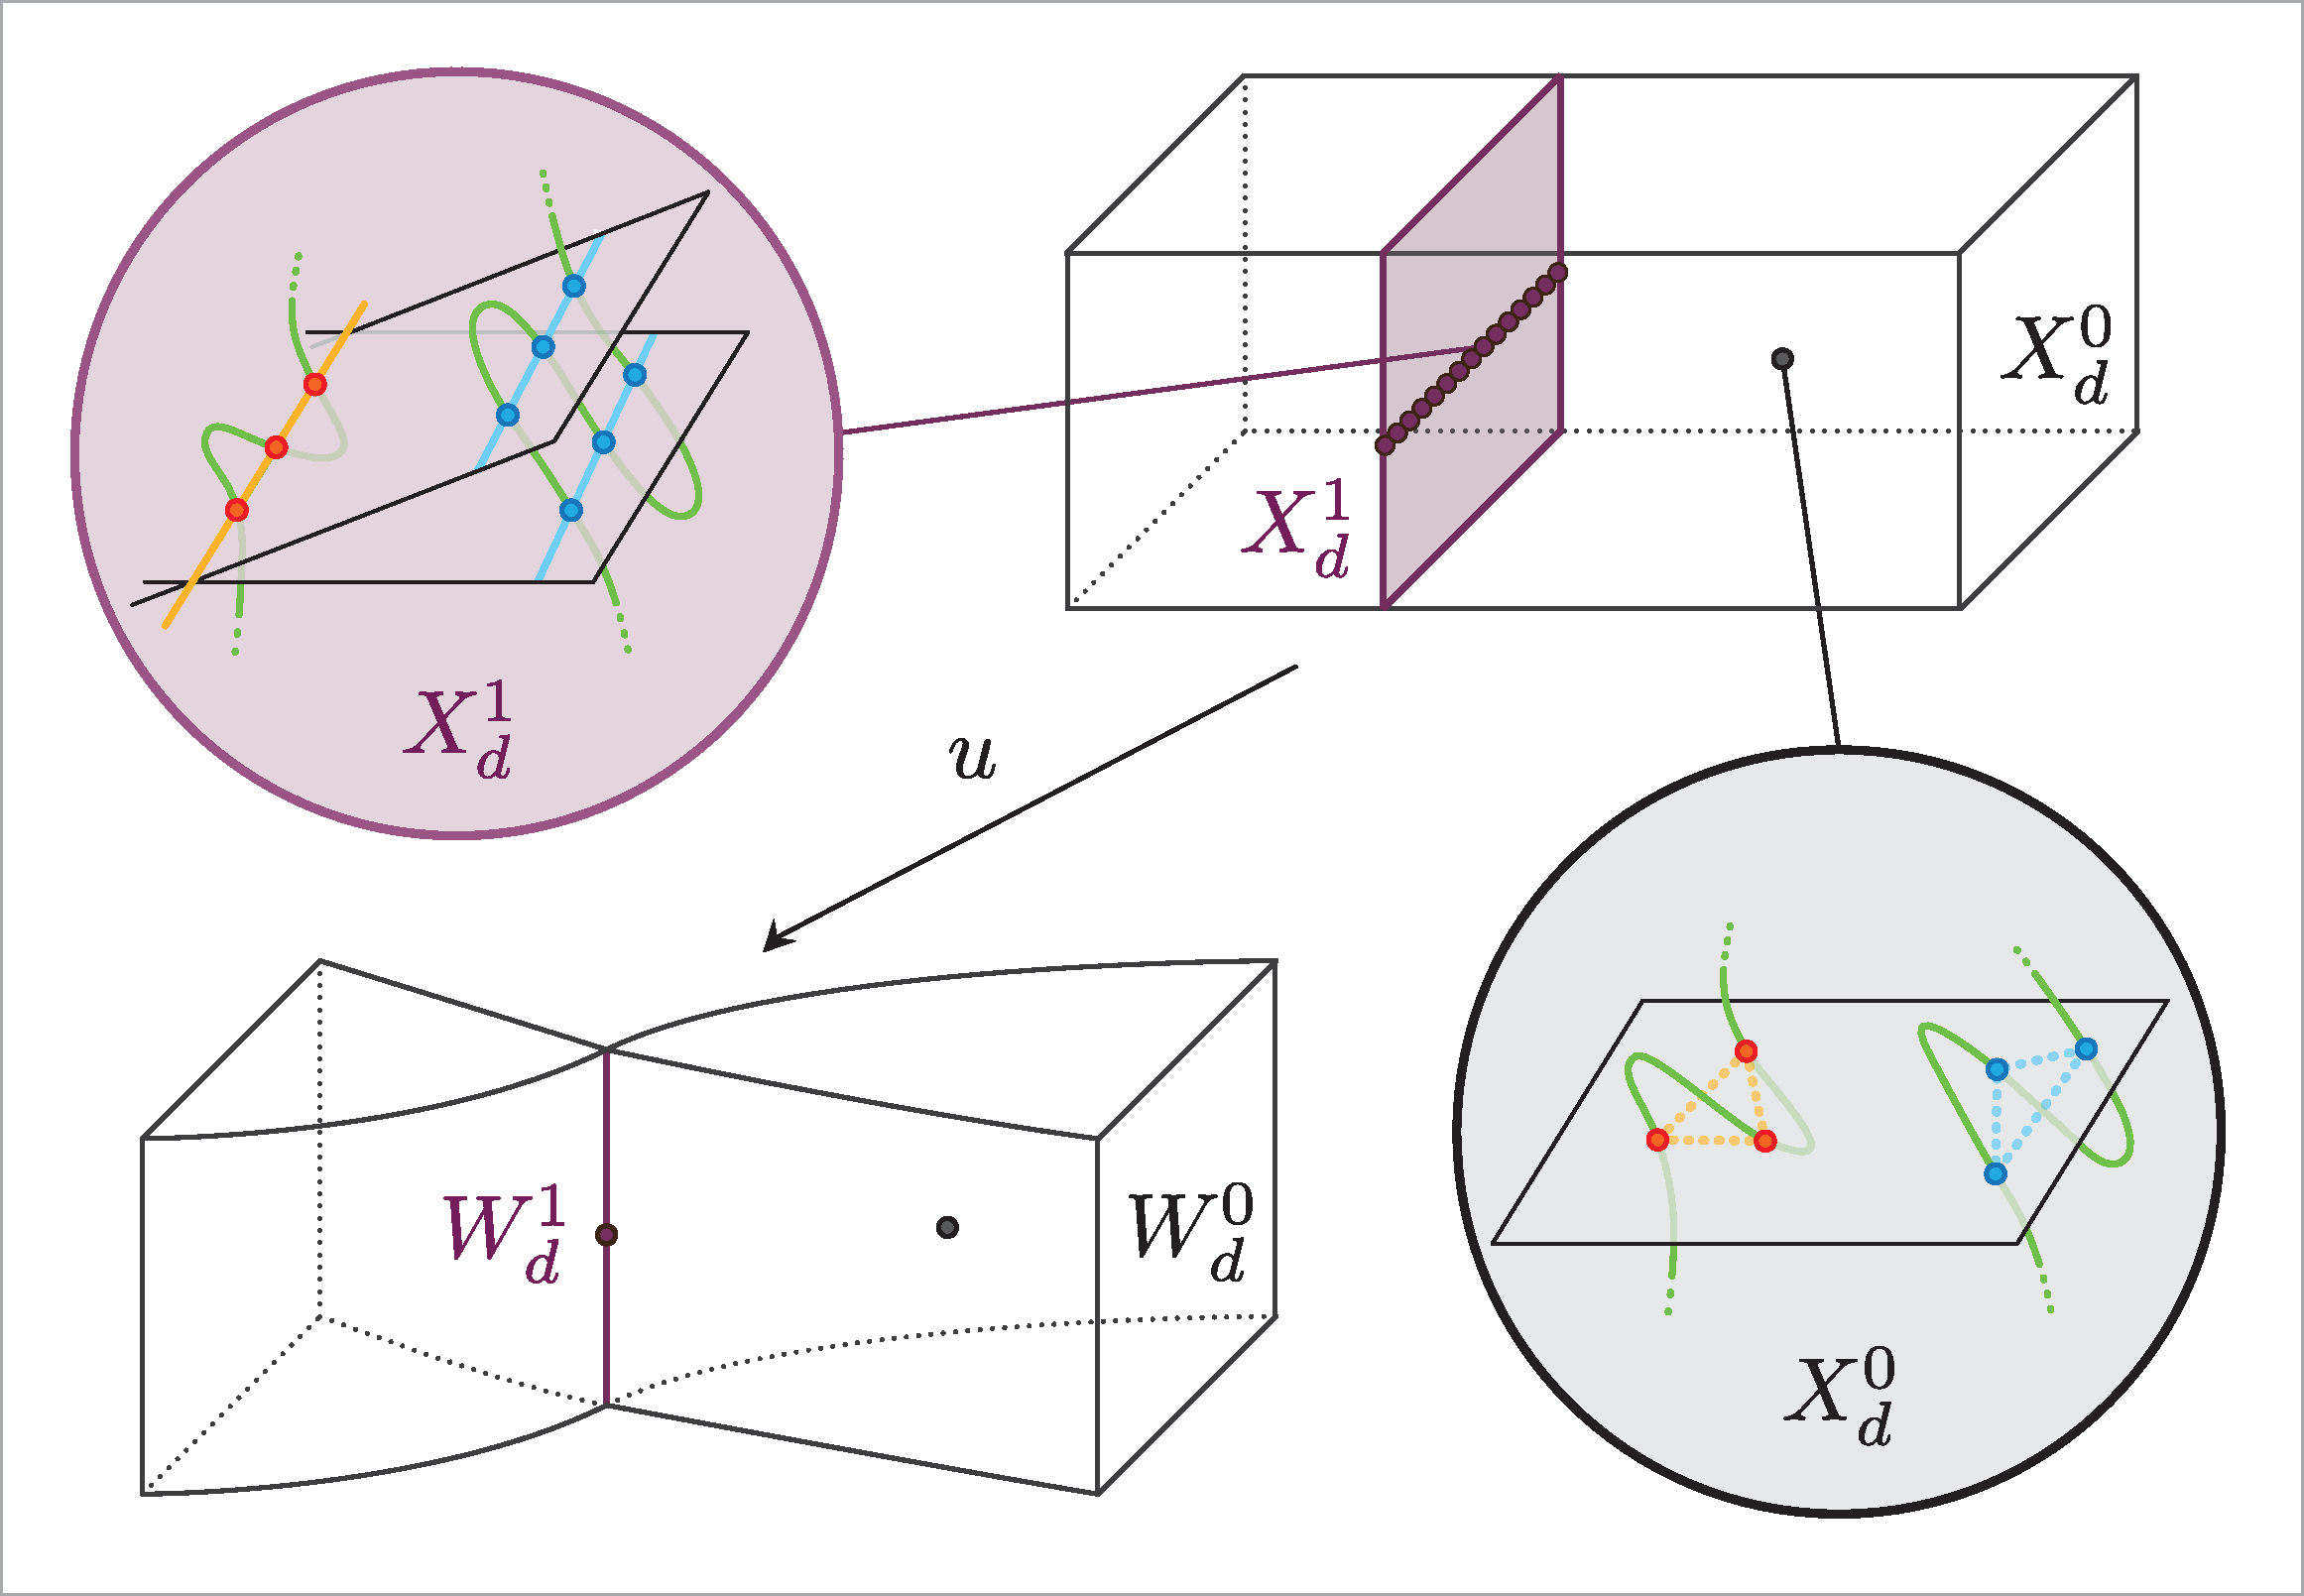
\includegraphics[width=\textwidth]{Degeneracy3.pdf}
		\caption{An intuitive picture of the Degeneracy loci of the Abel-Jacobi map $u$.}
	\end{figure}


\section{Dimensional lower bounds}\label{sec:lower_bound}
	%
	First of all let us introduce to the reader the so called \BN number, which will turn to be a crucial ingredient of \BN theory.
	\begin{defi}
		Let $d$, $g$ and $r$ be natural numbers. The \textbf{Brill-Noether number} is defined as
		$$\rho = \rho(d,g,r) = g - (r+1)(g-d+r)$$
	\end{defi}
	\vspace{1em}
	Let now $G$ be a finitely presented sheaf which admits the free presentation
	$$ E\overset{\ph}\to F \to G\to 0 $$
	with $E$ of rank $e$ and $F$ of rank $f$. Applying Theorem \ref{thm:height} to $G$ we get the inequality
	$$ \height (\Fitt_t(G)) \leq (e-f+t+1)(t+1). $$
	In the case of $\Xdr$, the sheaves appearing in the presentation \eqref{eq:univ_div_seq} have rank $d$ and $g$ as in \eqref{eq:e_f_k}. Hence, denoting by $I$ the (Fitting) ideal sheaf of $\Xdr$ we have
	$$ \height (I) \leq r(g-d+r). $$
	Since $\Dd$ is a variety over a field, it is a catenary scheme and we have the equality $ \codim \Xdr + \dim \Xdr = \dim \Dd $. Thus, recalling that $\dim \Dd = d$ we get the lower bound
	$$ \dim \Xdr \geq d - r(g-d+r) = g-(r+1)(g-d+r) + r = \rho + r $$
	for the dimension of every irreducible component of  $\Xdr$. Further, invoking Proposition \ref{prop:scheme_theo_inv_img} we deduce that any irreducible component of $\Wdr$ has dimension greater or equal than $\rho $. Let us state these results in the form of a Theorem, for future reference
	\begin{theo}\label{thm:lowerbounds}
		Every irreducible component of $\Xdr$ has dimension at least $ \rho + r$, while every irreducible component of $\Wdr$ has dimension at least $ \rho $.
	\end{theo}


\section{Definition of $\Gdr$}

	We are now going to define a variety $\Gdr$ parametrising $g_d^r$ on the curve $X$, i.e.\ (not necessarily complete) linear series of degree $d$ and dimension $r$. Our objective is to give the right definition for $\Gdr$ and then show that its support is given by
	$$ \Supp(\Gdr) = \set{ (L,W) \in \Pd \times \mathbb{G}(r+1, H^0(L)) } $$
	where $L$ is a line bundle on $X$ and $\mathbb{G}(r+1, H^0(L))$ denotes the Grassanian bundle of $(r+1)$-dimensional linear subspaces of $H^0(L)$.
	In order to give a scheme structure to $\Gdr$, we need to introduce a useful algebraic object. Let $G$ be a locally free and finitely presented sheaf over a scheme $Y$ and $ E\overset{\varphi}\to F \to G \to 0$ a free presentation of $G$, where $E$ and $F$ have finite ranks $e$ and $f$. Moreover, for every natural number $t\leq e$, let
	$$ \pi:\mathbb{G}(e-t, E)\to Y $$ 
	be the projection from the Grassmannian bundle of $(e-t)$-subspaces of sections of $E$ to $Y$.
	Consider the natural short exact sequence of sheaves over $\mathbb{G}(e-t, E)$
	$$ 0\to S \to \pi^* E \to Q \to 0 $$
	where $S$ and $Q$ are the universal subbundle and quotient bundle of $\mathbb{G}(e-t, E)$. 
	In order to better understand this sequence, let $y\in Y$ and let the $(e-t)$-subspace $V=\pi^{1}(y)$ be the corresponding fiber over $y$. Then the fiberwise \ses over $V$ is simply given by
	$$ 0\to V \to E_y \to E_y/V \to 0 \,. $$
	Next, we define the following subset of $\mathbb{G}(e-t, E)$ as a specific vanishing locus:
	\begin{defi}
		Ve define $\Grass_t(G) \subset \mathbb{G}(e-t, E)$ to be the vanishing locus of the morphism of sheaves
		$$ S\longrightarrow \pi^*E \overset{\pi^*\varphi} \longrightarrow \pi^* F $$
		i.e.\ the closed subset of the support of $\mathbb{G}(e-t, E)$ consisting of those points over which $S\to \pi^* F$ restricts to the zero morphism.
	\end{defi}
	\begin{rema}\label{rema:ker}
		Notice that, by definition, the support of $\Grass_t(G)$ consists of pairs $(y, V)$ where $y\in Y$ and $V\subset E_y$ is a $(e-t)$-subspace contained in the kernel of the linear map $\ph_y: E_y \to F_y$.
	\end{rema}
	Hence we can use the notion of $\Grass_t(\bullet)$ to define the variety $\Gdr$. To do so, first recall the definition of the high-degree divisor $\Gamma$ of degree $m$ as in Definition \ref{def:Gamma} and then consider the free presentation \eqref{eq:univ_lb_seq} of finite rank locally free sheaves over $\Pd$
	$$ \nu_{*} \scL(\Gamma)\overset{\gamma}\to R^1 \nu_{*} \scL(\Gamma) / \scL \to R^1 \nu_{*} \scL \to 0 $$
	which was involved in the definition of $\Wdr$.
	\begin{defi}
		We define $\Gdr$ to be the closed subscheme of $\mathbb{G}(r+1, \nu_{*} \scL(\Gamma))$ given by $\Grass_{(d+m-g+r)}(R^1 \nu_{*} \scL)$.
	\end{defi}
	One can show that the above definition is independent from the choice of the presentation of $R^1 \nu_{*} \scL$. We do not deal with this problem and we leave it as an exercise to the interested reader.\\

	It is now time to check that $\Gdr$ actually parametrizes $g_d^r$ on the curve. 
	First of all observe that, by Lemma \ref{lemm:functoriality}, the kernel of $\gamma_{\mid L}$ over any $L \in \Pd$ is canonically isomorphic to $H^0(L)$. 
	Therefore, looking at Remark \ref{rema:ker}, we see that the support of $\Gdr$ consists of couples $(L, W)$ where $L$ is a line bundle of degree $d$ and $W\subset H^0(L)$ is a linear subspace of dimension $r+1$, as desired.


\section{Cohomological description for the tangent spaces}

	In the following we will use the short hand notations
	$$ \Xdrr = \Xdr\setminus X_d^{r+1} \AND \Wdrr = \Wdr\setminus W_d^{r+1} $$
	and we will refer to the points of $\Xdrr$ and $\Wdrr$ as \textbf{good points}.\\
	With the aim of describing the tangent space of $\Wdr$ and $\Xdr$, we will first look at the one of $\Gdr$. A motivation for this approach is the observation that the natural projection
	$$ \beta:\Gdr\to\Wdr, \qquad (L,W) \mapsto L $$
	is biregular away of $W_d^{r+1}$. Indeed $\beta$ is clearly a regular map and, further, the preimage of $L\in \Wdrr$ consists just of the point $w=(L,H^0(L))$. It follows that, as far as $\Wdrr$ is regarded, $T\beta$ gives an isomorphism between the tangent spaces
	\begin{equation}\label{eq:tgnt_Wdrr}
		T\beta : T_{w}\Gdr \toiso T_L\Wdr, \quad \forall L\in\Wdrr.
	\end{equation}
	In order to describe the tangent space of $\Gdr$, a preliminary result about the first order deformations of a pair $(L,s) \in \Pic^d \times H^0(L)$ will turn out to be crucial.
	\begin{prop}\label{prop:cohom_condition}
		Let $L\in \Pic^d$ be a line bundle over $X$ and $s\in H^0(L)$ a global section. Then an element $\phi \in T_L\Pic^d \cong H^1(\OX)$ induces a first order deformation of the pair $(L,s)$ \ABiff $\phi\cdot s=0$ in $H^1(L)$.
	\end{prop}
	\begin{proof}
		Assume that $L$ is given by transition functions $g_\alb$ on a open cover $U_\al$ of $X$. We already know that $T_L \Pic^d \cong H^1(\OX)$ and a first order deformation $L'$ of $L$ is represented by a class $\phi \in H^1(\OX)$ in the following way
		$$ g_\alb \quad\overset{\phi}\leadsto\quad g'_\alb = g_\alb \cdot (1+ \eps \phi_\alb). $$  
		On the other hand, on a first order deformation of the pair $(L,s)$ to $(L',s')$ we have the additional requirement that the section $s'$ corresponds to a linear deformation of $s$. In formula this is expressed as
		$$ s'_\al = s_\al + \eps t_\al, \quad t \in H^0(L). $$
		The action of the transition functions can therefore be expanded as
		$$ s'_\beta = g'_\alb \cdot s'_\al \;\iff\; s_\beta + \eps t_\beta = g_\alb \cdot (1 + \eps \phi_\alb)\cdot(s_\al + \eps t_\al)$$
		and imposes the conditions
		$$ s_\beta = g_\alb \cdot s_\al \AND \phi_\alb \cdot s_\al = t_\al - g_{\beta\al}\cdot t_\beta. $$
		The first one is automatically satisfied since $s$ is a global section of $L$, while the second one can be rewritten in terms of the coboundary map $\partial : C^0(L) \to C^1(L)$ as
		$$ \phi \cdot s = \partial (t), $$
		thus giving the desired result.
	\end{proof}
	We now have a way to describe an element of $T_w\Gdr$. In fact the latter is nothing but a first order deformation of the pair $(L,W)$ and, as an immediate consequence of the above Proposition, one such deformation corresponds to an element $\phi\in H^1(\OX)$ such that $\phi\cdot W = 0$. Hence we deduce that the image of $T\beta$ at a point $w=(L,W)$ can be described as
	\begin{equation*}
		T\beta(T_w \Gdr) \cong \set{ \phi \in H^1(\OX) \mid \phi\cdot W = 0 \text{ in } H^1(L) }.
	\end{equation*}
	Further, this description can be reformulated using Serre's duality by considering the restriction of $\mu_0$ to $W\subseteq H^0(L)$, i.e.\ the map
	$$ \mu_{0,W} : W\otimes H^0(K-L) \to H^0(K), \quad s\otimes s' \mapsto s\cdot s'. $$
	Indeed, since the duality pairing is perfect, the condition $\phi\cdot W = 0$ is equivalent to require that $\forall s\in W$ and $\forall s'\in H^0(K-L)$ the pairing
	$$ \langle\, s',\, s\cdot \phi \, \rangle = \langle \,s'\cdot s,\, \phi \,\rangle $$
	vanishes. Notice that the above identity follows from Lemma \ref{lemm:pairing_properties} of Appendix A and the local description of abelian differentials. Therefore, in a more concise form, we can write 
	\begin{equation}\label{eq:im_beta_*}
		T\beta(T_w \Gdr)\cong(\,\im \mu_{0,W}\,)^{\vee}.
	\end{equation}

	As a consequence, at least for good points, we can easily describe the tangent space of $\Wdr$ in a purely cohomological fashion.
	\begin{prop}\label{prop:tgnt_Wdr}
		For every good point $L\in \Wdrr$ the tangent space is given by
		$$ T_L\Wdr \cong (\,\im \mu_{0}\,)^{\vee} $$
		where $ \mu_{0} : H^0(L)\otimes H^0(K-L) \to H^0(K) $ is the cup product.
	\end{prop}
	\begin{proof}
		This follows immediately from \eqref{eq:tgnt_Wdrr} and \eqref{eq:im_beta_*}, taking $W=H^0(L)$.\\
	\end{proof}
	Exploiting the fact that $\al$ is dual to $\delta$ we get, as a corollary, a nice cohomological description for the tangent space of $\Xdr$ as well.
	\begin{coro}\label{coro:tgnt_Xdr}
		For every good point $D\in \Xdrr$ the tangent space is given by
		$$ T_D\Xdr \cong (\,\im \al \mu_{0}\,)^{\vee} $$
		where $ \mu_{0} : H^0(D)\otimes H^0(K-D) \to H^0(K) $ is the cup product.
	\end{coro}
	\begin{proof}
		Let $D \in \Xdrr$ and set $L=u(D)$. Using Proposition \ref{prop:tgnt_Wdr} we find
		\begin{eqnarray*}
			T_D \Xdr 
			&=& u_{*}^{-1}\; T_L \Wdr \\
			&=& u_{*}^{-1}\: (\,\im \mu_0\,)^{\vee} \\
			&=& \delta^{-1}\; (\,\im \mu_0\,)^{\vee} \\
			&=& (\,\im \al \mu_0\,)^{\vee}
		\end{eqnarray*}
		where the last equality holds because $\al$ is dual to $\delta$, as shown in Appendix B -- see identity \eqref{eq:deltalpha}.
	\end{proof}


\section{Consequences of the infinitesimal study}

	We start with a proposition about the dimension of $\Gdr$. 
	\begin{prop}\label{prop:inf_Gdr}
		The dimension of $\Gdr$ is at least $\rho$ and, at every point $w=(L,W)$,  
		$$ \dim T_w \Gdr = \rho + \dim( \ker \mu_{0,W} ) .$$ 
		Hence $\Gdr$ is smooth of dimension $\rho$ at $w$ \ABiff $\mu_{0,W}$ is injective.
	\end{prop}
	\begin{proof}
		The lower bound on the dimension of $\Gdr$ follows directly from Theorem \ref{thm:lowerbounds}, since $\beta$ is onto $\Wdr$. To get the dimension of $T_w \Gdr$, notice that the fiber of $\beta$ over a point $L\in \Wdr$ is canonically isomorphic to the grassmanian $\mathbb{G}(r+1,H^0(L))$, whose tangent space at a point $W$ is given by $\Hom(W, H^0(L) / W)$. Hence we have a \ses
		$$ \SES{ \Hom(W, H^0(L) / W) }{ T_w \Gdr }{ \im (T\beta) } $$
		and the result follows from a trivial computation:
		\begin{eqnarray*}
			\dim T_w \Gdr
			&=& \dim\im(T\beta) + \dim\Hom(W, H^0(L) / W) \\
			&=& g-\dim\im\mu_{0,W} + (r+1)(h^0(L)-r-1) \\
			&=& g-(r+1)h^0(K-L) +\dim(\ker\mu_{0,W}) + (r+1)(h^0(L)-r-1) \\
			&=& g-(r+1)(h^0(K-L) - h^0(L)+r+1) +\dim(\ker\mu_{0,W}) \\
			&=& g-(r+1)(g-d+r) +\dim(\ker\mu_{0,W}) \\
			&=& \rho +\dim(\ker\mu_{0,W})
		\end{eqnarray*}
		The statement about the smoothness now follows immediately.
	\end{proof}
	As a corollary, we get an important result about the dimension and smoothness of $\Wdr$ at good points $L\in \Wdrr$.
	\begin{coro}
		The variety $\Wdr$ is smooth of dimension $\rho$ at $L\in \Wdrr$ \ABiff the cup product $ \mu_{0} : H^0(L)\otimes H^0(K-L) \to H^0(K) $ is injective.
	\end{coro}
	\begin{proof}
		From Proposition \ref{prop:inf_Gdr} together with \eqref{eq:tgnt_Wdrr} we know that for every good point $L$ 
		$$ \dim T_L \Wdr = \rho +\dim(\ker\mu_0) $$
		so it is enough to invoke the lower bound of Theorem \ref{thm:lowerbounds} to conclude.
	\end{proof}
	Finally, we have the corresponding result on the dimension and smoothness of $\Xdr$.
	\begin{prop}
		The variety $\Xdr$ is smooth of dimension $\rho+r$ at $D\in \Xdrr$ \ABiff the cup product $ \mu_{0} : H^0(D)\otimes H^0(K-D) \to H^0(K) $ is injective.
	\end{prop}
	\begin{proof}
		This is another a trivial computation. Indeed, using Corollary \ref{coro:tgnt_Xdr} and noticing that $\ker\al=H^0(K-D)$ is contained in the image of $\mu_0$, we get
			\begin{eqnarray*}
				\dim T_D \Xdr 
				&=& d - \dim\im\al\mu_0 = d - \dim\im\mu_0 + \dim\ker\al \\
				&=& d - (r+1)(g-d+r) + \dim\ker\mu_0  + g-d+r \\
				&=& r + g - (r+1)(g-d+r) + \dim\ker\mu_0 \\ 
				&=& r + \rho + \dim\ker\mu_0.
			\end{eqnarray*}
			The remark about the smoothness of $\Xdr$ at $D$ follows from the above combined with the lower bound of Theorem \ref{thm:lowerbounds}.
	\end{proof}
	{\color{Blue}
		This would be a good place to say something on the classical results about the injectivity of $\mu_0$ for a general curve.
	}
	\begin{comment}
		It would nice to show that at \textbf{bad} points the tangent cones are given by
		$$ T_D\Xdr \cong T_D\Dd \AND T_L\Wdr \cong T_L\Pd $$
		even if, most likely, time will not permit.
	\end{comment}
	





